% !TEX root = ../Thesis.tex

\subsection{Ampersand project}
In November 2003, the Business Rules Manifesto \citenac{business-rules} was written, with the main purpose of declaring independence for business rules in the world of requirements.
The manifesto supports the vision of business rules as equivalent to requirements.
This is considered a radical change on how people see the world of business architecture.

In December 2010, Stef Joosten, Lex Wedemeijer and Gerard Michels published the paper `Rule Based Design', presenting the Ampersand approach.
The approach puts the rules in the center, using these rules to define the business processes.
Ampersand is named after the \& symbol with the desire of realizing results for both business and IT, in an efficient and effective way.

In 2011, the Ampersand compiler was created as an open source project.
Since then, the compiler has been improved and applied in both business and academic contexts.
The Ampersand end-users write business rules in a specific language (ADL), and compile that specification into functional specification, documentation and working software prototypes.
\dict{ADL}{Ampersand Design Language}%
These rules are based on agreements between the different stakeholders.

The theory behind Ampersand has been thoroughly studied, and is based on mathe\-matical concepts, e.g. relational algebra and Tarski's axioms.
Using this compiler, users write the requirements in ADL and generate all the system specification independent of the platform.
The main advantage is that the requirement's consistency and traceability are always correct (and even provable), from the lowest level up to the front-end.
The requirements are presented to stakeholders in natural language, guaranteeing that any business expert who knows the context can validate the requirements.
\autoref{fig:generation} depicts the artifacts generated by the Ampersand compiler.
%
\begin{figure}[htb]
	\centering
	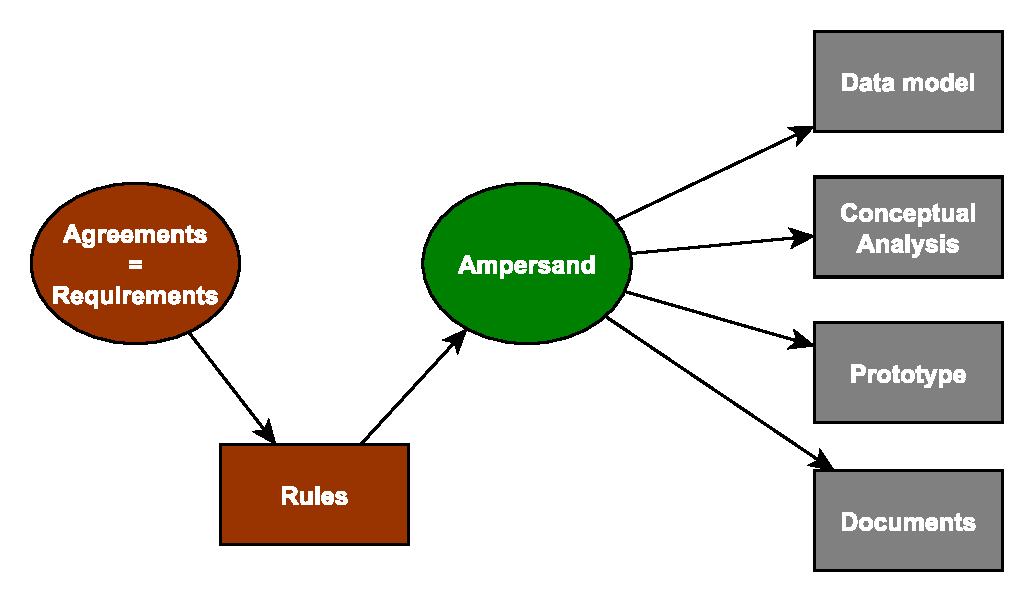
\includegraphics[width=0.7\textwidth]{Figures/Generation}
	\caption[Generated artifacts]{The Ampersand approach generates different artifacts based on the business rules (source: \cite{ampersand-approach})}
	\label{fig:generation}
\end{figure}
%

The Ampersand project is used in several environments, by different user groups.
In a research context, the Ampersand project is part of the research on the use of business rules for software design.
In an academic context, it is also used as the main tool in the course `Ontwerpen met bedrijfsregels' (code T18321) from the Open University of the Netherlands.
Finally, the compiler is used in business environments to design and develop real world business software.
